%\begin{frame}
%	\frametitle{Google Map API}
%%
%	\begin{block}{Implementierung in GUI}
%		\begin{itemize}
%			\item Es existiert nur eine API für \textit{Andriod}
%			\item Workaround über Browser möglich
%			\item Ansatz: Firefox in GUI integrieren
%			\item Problem: Bläht das Programm \textbf{enorm} auf
%		\end{itemize}
%	\end{block}
%%
%	\begin{block}{Kommunikation zu SM}
%		\begin{itemize}
%			\item Problem dem Scrum Master erläutert
%			\item Klärung mit Product Owner erforderlich
%		\end{itemize}
%	\end{block}
%\end{frame}
%
%
%
\begin{frame}
	\frametitle{Lageplan der Hochschule}
%
	\begin{block}{Implementierung in GUI}
		\begin{itemize}
			\item Lageplan kann als Bild hinterlegt werden
			\item Einfache Wartung möglich
			\item Anzeige über die Klasse Image
		\end{itemize}
	\end{block}
\end{frame}
%
%
%
\begin{frame}
	\frametitle{Interaktive Liste}
%
	\begin{minipage}{0.49\textwidth}
		\begin{figure}
			\centering
			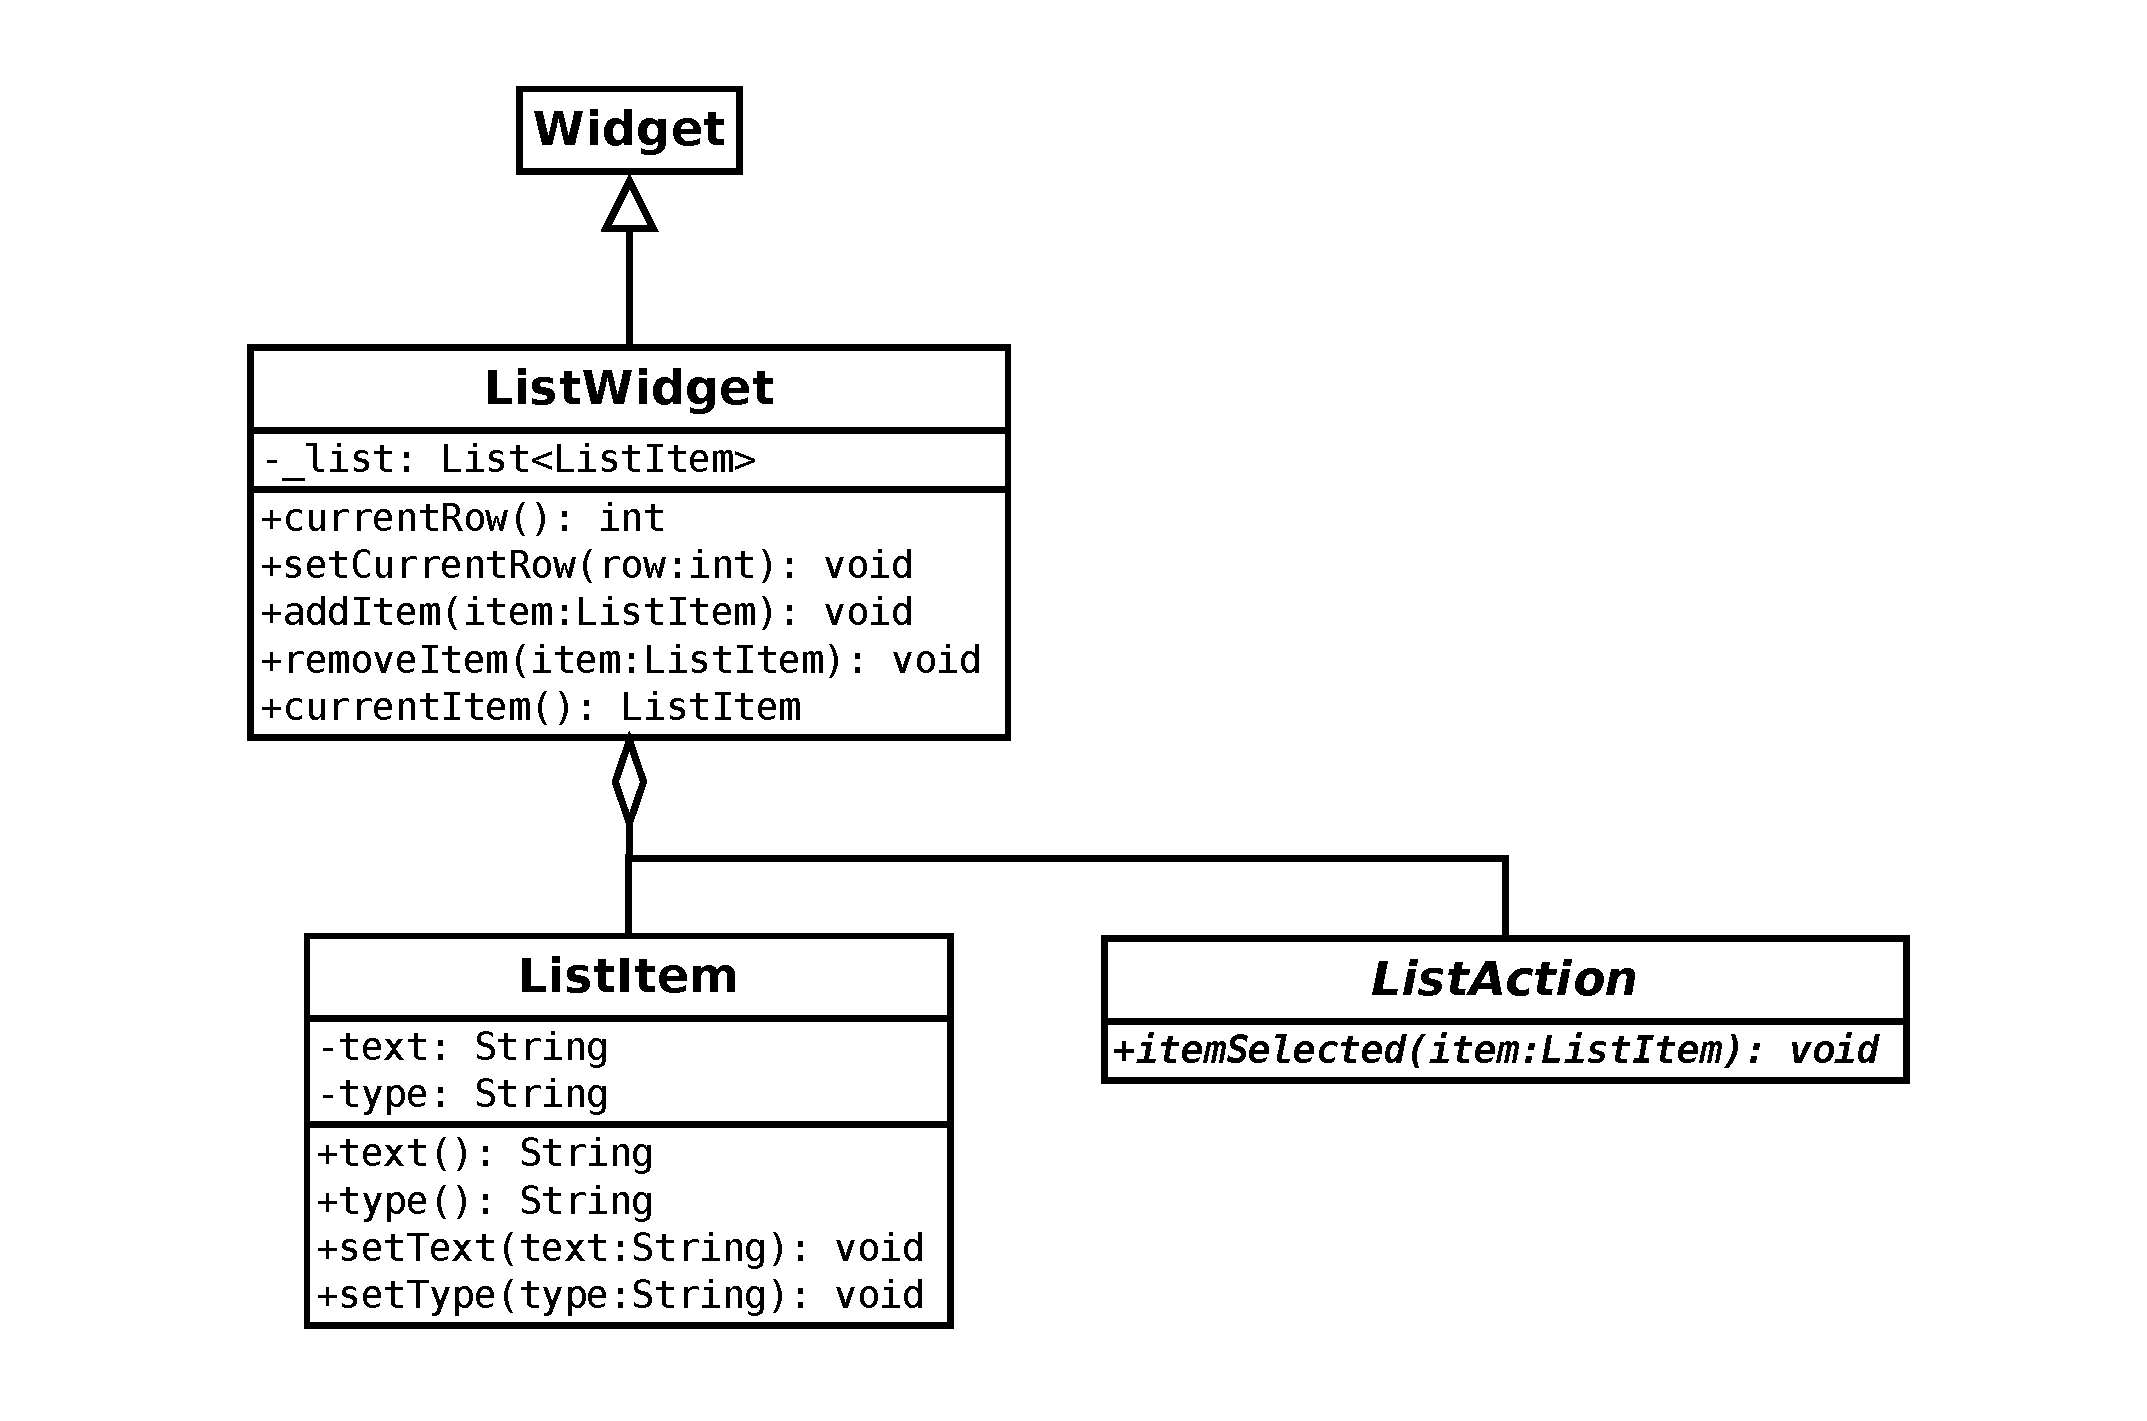
\includegraphics[width = \textwidth]{../grafiken/uml-list-widget}
			\caption{UML Diagram ListWidget}
		\end{figure}
	\end{minipage}
%
	\begin{minipage}{0.44\textwidth}
		\begin{block}{ListItem}
			\begin{itemize}
			    \item Erbt von Widget
			    \item ListAction ist das Interface zum Model
			    \item ListItem enthält alle Daten für ein Item
			    \item Leicht erweiterbar
			\end{itemize}
		\end{block}
	\end{minipage}
\end{frame}